
Ce chapitre présente le début de nos travaux toujours en cours 
sur le problème de la synthèse de mouvements par optimisation.
D'une part en optimisant un critère de stabilité et d'énergie, 
calculé à l'aide du modèle dynamique inverse du robot.
D'autre part, en implémentant un simulateur physique (dynamique directe) 
capable de prendre en compte les imperfections du robot.
La première section détaille les notions de modélisation
dynamique nécessaires à la fois au calcul du critère de stabilité 
et également à la simulation du robot en contact avec le sol.
La deuxième section présente la méthode de synthèse de mouvements
de tir expérimentée et évoque rapidement sans les détailler 
nos premiers résultats.

\section{Modélisation et calculs Dynamiques\label{sec:model_dynamics}}

\subsection{Motivations}

Cette partie présente succinctement les différents
concepts classiques permettant d'appréhender le comportement
dynamique des systèmes robotiques, avec et sans présence de contacts.
Ces concepts sont basés sur la théorie des solides rigides
(\textit{rigid body dynamics}),
extension aux systèmes polyarticulés de la théorie mécanique de Newton.

La modélisation dynamique d'un système mécanique
établie les relations entre les accélérations (variation du mouvement) 
de chaque degré de liberté et les forces qui leurs sont appliquées.
Elle permet de décrire l'évolution temporelle
du système et d'expliquer les causes du mouvement.

L'objectif pratique est double. 
Premièrement, être capable à partir de la définition d'un mouvement,
de quantifier sa qualité (consommation énergétique, stabilité, 
voir section \ref{sec:motion_fitness}).
Ceci afin de pouvoir construire par optimisation la forme d'un mouvement
idéal en supposant \og parfait \fg (sans défaut), la dynamique du robot.
Deuxièmement, l'implémentation d'un simulateur
capturant le mieux possible le comportement dynamique réel du robot 
(voir section \ref{sec:motion_simulation}).
L'idée est alors d'appliquer une approche similaire à celle présentée
section \ref{sec:odometry_cmaes} pour l'optimisation d'une politique de contrôle
de la marche avec l'apprentissage de odométrie prédictive.
Après identification expérimentale des paramètres du simulateur,
l'ambition est la correction (raffinement) d'un mouvement (en boucle ouverte pour commencer)
par optimisation au sein du simulateur.
Ceci dans le but de prendre en compte 
(par pré-compensation) les imperfections du robot tout en limitant 
autant que possible les expérimentations sur le robot physique.

Les notations et les équations de cette section sont
directement tirées du livre de référence de
Roy Featherstone, \cite{featherstone_rigid_2008}.
Cet ouvrage m'a beaucoup apporté, notamment en ce qui concerne
la compréhension des contacts et la dynamique 
du double support du robot.

\subsection{Paramètres inertiels}

Chaque solide du robot est dynamiquement caractérisé 
par les $10$ paramètres suivants :
\begin{itemize}
    \item Sa masse ($1$ paramètre).
    \item La position de son centre de masse ($3$ paramètres).
        Cette position est généralement exprimée dans le repère lié au solide.
    \item Les coefficients définissant sa matrice d'inertie 
        au centre de masse ($6$ paramètres).
\end{itemize}
L'ensemble de ses paramètres pour tous les solides du robot 
(ainsi que la topologie mécanique) forment le modèle dynamique.
La matrice d'inertie est pour rappel une matrice carrée symétrique de taille $3$
s'exprimant :
$$
\bm{I} =
\begin{bmatrix}
    I_{xx} & I_{xy} & I_{xz} \\
    I_{xy} & I_{yy} & I_{yz} \\
    I_{xz} & I_{yz} & I_{zz} \\
\end{bmatrix}
$$

Une estimation approximative de ces paramètres peut être fournie par 
un assemblage virtuel du robot dans un outil de conception assisté 
par ordinateur des pièces mécaniques.
Il faut néanmoins préciser la masse connue des différents composants
ainsi que de la matière aluminium utilisée.
Malheureusement, il subsiste un écart de l'ordre de $1$~Kg (sur un total
de $4.2$~Kg) entre la 
masse obtenue et le poids réellement mesuré sur le robot.
Cette \og masse manquante \fg provient du poids du câblage et
de la visserie en acier.
Pour faire correspondre les deux masses, la masse volumique
de l'aluminium est artificiellement augmentée.
Les valeurs des paramètres inertiels ne sont donc connues
que approximativement, même en supposant la géométrie non déformée.

\subsection{Modèles de la dynamique\label{sec:dynamics_models}}

\begin{definition}
    Soit respectivement le vecteur des positions, vitesses et accélérations articulaires 
    noté $\bm{q},\bm{\dot{q}},\bm{\ddot{q}} \in \mathbb{R}^n$ de tous les $n$ degrés de 
    liberté du système.
    Soit également le vecteur des couples articulaires $\bm{\tau} \in \mathbb{R}^n$ exercés 
    sur ces degrés de liberté.\\
    Le modèle dynamique direct du système se défini par la procédure de calcul suivante :
    $$\mathsf{FD} :~ (\bm{q}, \bm{\dot{q}}, \bm{\tau}) \longmapsto \bm{\ddot{q}}$$
    Le modèle dynamique inverse du système se défini par la procédure de calcul suivante :
    $$\mathsf{ID} :~ (\bm{q}, \bm{\dot{q}}, \bm{\ddot{q}}) \longmapsto \bm{\tau}$$
\end{definition}

Dans un premier temps, on considère le cas le plus simple 
où le robot est en simple support.
Un seul de ses pieds est en contact avec le sol.
De plus, la racine de l'arbre mécanique est positionnée au
niveau du centre du pied de support.
La topologie du robot se réduit donc à un arbre (pas de boucle cinématique) dont
la racine est fixée par rapport au sol (pas de glissement).
Dans cette configuration, les modèles dynamiques direct et inverse
sont des fonctions bien définies et n'admettent qu'une et une seule solution.\\

Deux grands types d'algorithmes dynamiques sont ici à l'oeuvre.
Dans le cas \textit{simple}, les algorithmes classiques en $\mathcal{O}(n)$ 
(avec $n$ le nombre de degrés de liberté du système), 
s'appliquent et fonctionnent par propagation montante et descendante
de valeurs numériques le long de l'arbre.
D'un autre coté, on trouve également les algorithmes en $\mathcal{O}(n^3)$
formant et résolvant directement l'équation du mouvement dans sa
forme matricielle. 
Plus couteux, l'intérêt de ces derniers est de pouvoir gérer 
les cas plus complexes de contacts. 

Dans ces travaux, les algorithmes en $\mathcal{O}(n)$ sont utilisés
lorsque le robot est explicitement en permanence en simple support.
Lors des autres cas, les algorithmes en $\mathcal{O}(n^3)$
sont préférés ; même si parfois, une gestion plus fine en alternant entre
les deux types d'algorithmes permettrait de gagner 
en temps de calcul\footnote{De la même manière, le caractère creux (\textit{sparse})
de certaines matrices n'est pas ici exploitée et représenterait une amélioration 
de l'implémentation.}.\\

Les trois algorithmes classiques en $\mathcal{O}(n)$ sont les suivants :
\begin{itemize}
    \item Algorithme de Newton-Euler récursif (\textit{recursive Newton-Euler algorithm}).\\
        Cette procédure résout le modèle dynamique inverse d'un robot polyarticulé
        dans le cas simple d'une topologie mécanique en arbre.
    \item Algorithme des solides articulés (\textit{articulated-body algorithm}).\\
        Toujours dans le cas simple, cet algorithme calcul le modèle
        dynamique direct d'un robot polyarticulé.
    \item Algorithme des solides composés (\textit{composite rigid body algorithm}).\\
        Cet algorithme calcul la matrice d'inertie $\bm{H}$ présentée ci-dessous.
    \newline
\end{itemize}

Les équations de la dynamique d'un système sous la forme
d'un arbre mécanique s'écrivent sous la forme matricielle suivante.
L'intérêt de cette forme est qu'elle travaille directement
dans l'espace articulaire. 
Contrairement aux simulateurs physiques 
\og généralistes \fg\footnote{Par exemple, \textit{Bullet} et \textit{ODE}}
(résolution d'équations différentielles sous contraintes),
les contraintes générées par les articulations
sur le mouvement du système mécanique sont ici \textbf{implicites} :

$$
\bm{H}(\bm{q})\bm{\ddot{q}} + \bm{C}(\bm{q}, \bm{\dot{q}}) = \bm{\tau}
$$

où $\bm{q}, \bm{\dot{q}}, \bm{\ddot{q}}, \bm{\tau} \in \mathbb{R}^{n}$ 
sont respectivement le vecteur des positions, vitesses, accélérations 
et des couples de chacun des $n$ degrés de liberté du système.
La matrice diagonale, symétrique et définie positive $\bm{H} \in \mathbb{R}^{n \times n}$ 
est appelée matrice d'inertie articulaire (\textit{joint-space inertia matrix}).
Elle ne dépend que des positions ($\bm{q}$) et représente l'effet des masses du système.
Enfin, le vecteur $\bm{C} \in \mathbb{R}^{n}$ est appelé, vecteur des forces articulaires
(\textit{joint-space bias force}).
Il dépend à la fois des positions et des vitesses angulaires ($\bm{q},\bm{\dot{q}}$) 
et représente les forces (gravité, Coriolis) s'appliquant au système,
converties dans l'espace articulaire.\\

La matrice $\bm{H}$ se calcule en $\mathcal{O}(n)$ directement avec 
l'algorithme des solides composés. 
Le vecteur $\bm{C}$ s'obtient également en $\mathcal{O}(n)$ par application
du modèle dynamique inverse, calculé par l'algorithme de Newton-Euler récursif :

$$
\bm{C}(\bm{q}, \bm{\dot{q}}) = 
\mathsf{ID}(\bm{q}, \bm{\dot{q}}, \bm{0})
$$

À partir de l'équation du mouvement, le modèle dynamique direct
peut se calculer en $\mathcal{O}(n^3)$ par résolution de l'équation : 

$$
\bm{\ddot{q}} = \bm{H}^{-1}\big(\bm{\tau} - \bm{C}\big)
$$

\subsection{Modélisation des contacts}

Lorsque le robot a ses deux pieds en contact avec le sol,
la topologie du système mécanique ne forme plus un arbre.
En supposant qu'il n'y a pas de glissement\footnote{L'étude de la
dynamique des robots en présence de contacts et de glissements est
un domaine actif de recherche. On peut par exemple mentionner les travaux de
Evan Drumwright sur la dynamique inverse d'un robot quadrupède 
en présence de glissements (\cite{zapolsky_inverse_2017}).},
les deux pieds ne peuvent alors plus bouger l'un par rapport.
Cette situation créée une boucle cinématique fermée entre les deux jambes ; 
le sol faisant alors comme partie de la structure du robot.
Cette boucle limite les mouvements de la chaine des articulations.
Elle est ainsi mathématiquement modélisée par la notion 
de contraintes cinématiques.\\

\begin{definition}
    On note $n \in \mathbb{N}$ le nombre de degrés de liberté du système 
    et $m \in \mathbb{N}$ le nombre de contraintes cinématiques.
    Soit $\bm{\ddot{q}} \in \mathbb{R}^{n}$ le vecteur des accélérations
    des articulations.
    Les $m$ contraintes cinématiques sont définies au niveau de l'accélération
    et dans l'espace articulaire par la matrice rectangulaire 
    $\bm{K} \in \mathbb{R}^{m \times n}$ et le vecteur $\bm{k} \in \mathbb{R}^{m}$ 
    tels que :
    $$
    \bm{K}\bm{\ddot{q}} = \bm{k}
    $$
\end{definition}

En pratique, la matrice $\bm{K}$ est construite par
concaténation en lignes des matrices jacobiennes (avec ou sans les orientations)
calculées aux différents points de contacts considérés.

Par exemple, dans le cas où le robot est en double support et
les deux pieds à plat sur le sol, l'un des pieds est choisi
comme base flottante de l'arbre mécanique (fixe dans le monde).
On souhaite exprimer le fait que le centre de l'autre pied reste fixe 
par rapport au premier pied de support.
Soit $\bm{J}_{\text{pied}} \in \mathbb{R}^{6 \times n}$ la jacobienne 
du centre du deuxième pied.
À noter que cette jacobienne utilise la notation de Plücker en considérant
les translations (vecteur vitesse linéaire) mais également 
les rotations (vecteur vitesse de rotation angulaire) cartésiennes. 
Par définition :
$$
\begin{bmatrix}
    \omega_\text{x} \\
    \omega_\text{y} \\
    \omega_\text{z} \\
    v_\text{x} \\
    v_\text{y} \\
    v_\text{z} \\
\end{bmatrix}
= \bm{J}_{\text{pied}}(\bm{q}) . \bm{\dot{q}}
$$
Donc pour exprimer un mouvement nul, autant en translation qu'en rotation 
($m=6$ contraintes) il faut que : 
$$
\bm{J}_{\text{pied}}\bm{\dot{q}} = \bm{0}
$$
Soit au niveau des accélérations : 
$$
\bm{J}_{\text{pied}}\bm{\ddot{q}} + \bm{\dot{J}}_{\text{pied}}\bm{\dot{q}} = \bm{0}
$$
on a donc ici $\bm{K} = \bm{J}_{\text{pied}}$ et 
$\bm{k} = -\bm{\dot{J}}_{\text{pied}}\bm{\dot{q}}$.\\

On note $\bm{\lambda} \in \mathbb{R}^{m}$ le vecteur des 
\og forces de contraintes \fg cartésiennes représentant l'action 
des contraintes cinématiques sur la dynamique du robot.
Chacune des forces agit pour faire respecter la contrainte
auquel elle est associée.
Par exemple, la force de contre réaction du sol assure que la contrainte
de non interpénétration soit respectée.
Dans l'espace angulaire, ces forces agissent
sur chaque articulation sous la forme d'un vecteur de \og couples de contraintes \fg
$\bm{\tau}_{c} \in \mathbb{R}^{n}$ donné par :
$$
\bm{\tau}_{c} = \bm{K}^\T \bm{\lambda}
$$
\newline

En réalité, seul un sous ensemble de toutes les contraintes cinématiques possibles
($3~\times$ nombre de points de contact) est
réellement inclus dans la définition de la matrice $\bm{K}$.
En effet, il est essentiel pour éviter les instabilités numériques
lors de la résolutions des équations matricielles, de ne pas introduire
de contraintes redondantes.
Pour chaque pied un maximum de $6$ contraintes sont créés.
Pour le calcul de la dynamique inverse en double support, 
$6$ contraintes de positions et orientations bloquent 
complètement le mouvement du pied.
Dans le cas de la simulation, plusieurs cas se présentent :
\begin{itemize}
    \item Si un seul crampon est en contact avec le sol,
        seuls $3$ contraintes (de positions) sont utilisées.
    \item Si deux crampons sont en contact, le pied possède encore
        un degré de liberté en roulement et $5$ contraintes sont donc définies.
    \item Enfin, quand les quatre crampons sont posés sur le sol, 
        la totalité des $6$ contraintes (de positions) sont imposées.
\end{itemize}
Chacun des crampons en contact avec le sol définit toujours 
au moins une contrainte verticale.
Les autres contraintes tangentielles (parallèles au plan du sol) 
sont ajoutées afin d'atteindre le bon nombre de contraintes.
Il faut cependant assurer que les lignes d'action de ces forces de contraintes
tangentielles ne soit pas confondues.
Ceci afin d'éviter que des forces de contraintes puissent 
\og lutter \fg numériquement l'une contre l'autre.

\subsection{Dynamique et contraintes cinématiques\label{sec:dynamics_constraints}}

En ajoutant les couples de contraintes
à l'équation de la dynamique, on obtient le système suivant :
$$
\begin{cases}
\bm{H}\bm{\ddot{q}} + \bm{C} - \bm{K}^\T\bm{\lambda} = \bm{\tau} \\
\bm{K}\bm{\ddot{q}} = \bm{k}
\end{cases}
$$
qui se reformule sous forme matricielle pour donner l'équation
de la dynamique du robot sous contraintes cinématiques :
$$
\begin{bmatrix}
    \bm{H} & \bm{K}^\T \\
    \bm{K} & \bm{0} \\
\end{bmatrix}
\begin{bmatrix}
    \bm{\ddot{q}} \\
    -\bm{\lambda} \\
\end{bmatrix}
=
\begin{bmatrix}
    \bm{\tau} - \bm{C} \\
    \bm{k} \\
\end{bmatrix}
$$

À partir de cette équation, le modèle dynamique direct
du robot sous contraintes peut être résolu directement avec
une complexité en $\mathcal{O}((n+m)^3)$:
$$
\begin{bmatrix}
    \bm{\ddot{q}} \\
    -\bm{\lambda} \\
\end{bmatrix}
=
\begin{bmatrix}
    \bm{H} & \bm{K}^\T \\
    \bm{K} & \bm{0} \\
\end{bmatrix}^{-1}
\begin{bmatrix}
    \bm{\tau} - \bm{C} \\
    \bm{k} \\
\end{bmatrix}
$$

À noter qu'en pratique, la matrice n'est pas directement inversée.
Une décomposition \textit{QR} par la méthode du pivot de Householder
est réalisée ($\bm{H} = \bm{P}^{-1}\bm{Q}\bm{R}\bm{P'}^{-1}$).
Cette décomposition, implémentée par la bibliothèque d'algèbre 
linéaire \textit{Eigen}, assure une meilleure stabilité 
numérique des calculs.\\

De la même manière que le modèle géométrique inverse 
est mal défini dans le cas général, le modèle dynamique inverse
d'un système mécanique ayant au moins un boucle cinématique fermée 
admet une infinité de solutions.
Par exemple lorsque le robot est immobile en double support, 
il peut soit ne compenser que la gravité, soit faire que ses
jambes poussent latéralement dans des sens opposés et créant 
des forces qui se neutralisent.
Dans les deux cas, les positions, vitesses et accélérations
des articulations sont les mêmes alors que les forces ressenties 
sont différentes.
Les calculs ci dessous permettent d'accéder à ces solution.

On note $r \in \mathbb{N}$ le rang de la matrice $\bm{K} \in \mathbb{R}^{m \times n}$.
Soit $\bm{G} \in \mathbb{R}^{n \times (n-r)}$ la matrice telle que : 
$$
\bm{K}\bm{G} = \bm{G}^\T\bm{K}^\T = \bm{0} \in \mathbb{R}^{m \times (n-r)}
$$
La matrice $\bm{G}$ est formée des vecteurs colonnes composant 
la base du noyau (kernel) de $\bm{K}$.
Elle est calculée au travers d'une décomposition
\textit{LU} de la matrice $\bm{K}$ ($\bm{K} = \bm{P}^{-1}\bm{L}\bm{U}\bm{Q}^{-1}$).

En multipliant l'équation de la dynamique par $\bm{G}^\T$, 
le terme contenant $\bm{\lambda}$ est éliminé :
$$
\bm{G}^\T \big(\bm{H}\bm{\ddot{q}} + \bm{C}\big) = \bm{G}^\T \bm{\tau}
$$
On reconnait alors à gauche de l'égalité le vecteur des couples 
calculé à partir du modèle dynamique inverse simple (sans contrainte) 
$\bm{\tau}_{\text{ID}} \in \mathbb{R}^{n}$ : 
$$
\underset{\scriptscriptstyle (n-r) \times 1}{\bm{G}^\T \bm{\tau}_{\text{ID}}}
= 
\underset{\scriptscriptstyle (n-r) \times n}{\bm{G}^\T} ~~
\underset{\scriptscriptstyle n \times 1}{\bm{\tau}}
$$
Dès que le rang $r$ de la matrice $\bm{K}$ est non nulle, c'est à dire
dès qu'au moins une contrainte cinématique est réellement définie, ce système
devient sous contraint. Il possède alors une infinité de solutions.

Le choix a été fait de sélectionner parmi toutes les solutions possibles, 
la solution aux moindres carrés ; minimisant la norme euclidienne 
du vecteur des couples. 
Ceci a l'avantage d'éviter les cas \og dégénérés \fg où deux 
ensembles de couples infiniment grand se compensent.
Le système est ainsi résolu au moyen d'une pseudo inverse,
calculée à l'aide d'une décomposition \textit{SVD}.

À noter qu'il est important lors de la résolution du système
par la pseudo inverse de ne pas prendre en compte les degrés
de liberté associés à la base flottante.
En effet, la base flottante comprend notamment $3$ valeurs de translation.
Les ordres de grandeurs de ces distances sont très différents de ceux
des angles des articulations.
Ils doivent ainsi être éliminés pour ne pas biaiser la minimisation 
de la norme euclidienne.

\subsection{Définition et calcul du ZMP\label{sec:zmp}}

Le ZMP ou \textit{Zero Moment Point} (\cite{vukobratovic_zero-moment_2004})
est un point dynamique abondamment utilisé comme critère de stabilité
pour la locomotion bipède.
Il se définit sur un sol plat comme le point où la résultante des forces 
du système mécanique sur le sol ne produit aucun moment horizontal.

Soit $O$ un point sur le sol, par exemple le centre du pied de support du robot.
On note $\bm{F}_{O} \in \mathbb{R}^{3}$ et $\bm{M}_{O} \in \mathbb{R}^{3}$
respectivement la résultante des forces et des moments exercées par le système
mécanique sur le sol au niveau du point $O$ :
$$
\bm{F}_{O} = 
\begin{bmatrix}
    f_{\text{x}} \\
    f_{\text{y}} \\
    f_{\text{z}} \\
\end{bmatrix},~
\bm{M}_{O} = 
\begin{bmatrix}
    \tau_{\text{x}} \\
    \tau_{\text{y}} \\
    \tau_{\text{z}} \\
\end{bmatrix}
$$
En supposant le sol plat et en notant $\vec{n}$ la normale au sol,
le point ZMP noté $P$ s'exprime par définition de la manière suivante : 
$$
\vec{OP} = \frac{\vec{n} \times \bm{M}_{O}}{\vec{n} . \bm{F}_{O}}
$$
Dans le repère du point $O$, le vecteur des coordonnées du ZMP
s'exprime donc : 
$$
\bm{ZMP}_{O} = 
\begin{bmatrix}
    -\frac{\tau_{\text{y}}}{f_{\text{z}}} \\
    \frac{\tau_{\text{x}}}{f_{\text{z}}} \\
    0 \\
\end{bmatrix}
$$

Les forces latérales $f_{\text{x}}$ et $f_{\text{y}}$ ainsi que
le couple en torsion $\tau_{\text{z}}$ ne sont pas considérés.
En effet, il est ici supposé que les frottements sont suffisants
pour s'opposer à tout glissement et à toute rotation du pied 
du robot sur le sol.

Les forces et couples résultants $\bm{F}_{O}$ et $\bm{M}_{O}$ sont
en pratique calculés à l'aide du modèle dynamique inverse en simple support.
En considérant que la base flottante du système mécanique est placée au niveau 
du pied de support du robot et que ce dernier est à plat sur le sol, 
le vecteur des forces agissant sur les 
six degrés de liberté de la base est précisément :
$$
\begin{bmatrix}
    \bm{M}_{O} \\ 
    \bm{F}_{O} \\
\end{bmatrix} \in \mathbb{R}^{6}
$$
Pour rappel, la base flottante permet de déplacer le modèle du robot dans
le monde cartésien. Il s'agit de degrés de liberté placés entre la vrai
base à l'origine du monde et la racine de l'arbre mécanique du robot
(voir la section \ref{sec:modele_topologie}).
Le calcul du ZMP par le modèle dynamique inverse simple 
($\mathsf{ID}(\bm{q}, \bm{\dot{q}}, \bm{\ddot{q}}) = \bm{\tau}$) nécessite donc
la connaissance des positions, vitesses et accélérations des articulations
du système.

On peut prouver que quand le robot est en phase de double support, 
le calcul du ZMP est en réalité identique.
Même si les deux pieds du robot sont en contact avec le sol,
un pied est arbitrairement choisi comme pied de support.
La dynamique inverse est alors calculée comme si le robot
était en simple support, et les valeurs des forces et couples
des articulations de la base flottante sont utilisées pour déterminer le ZMP.
Intuitivement, que les forces et couples appliqués par le robot sur le sol
soient concentrés au niveau d'un point, ou répartis sur les deux pieds,
la résultante de l'action du système une fois reportée dans un même 
référentiel est la même\footnote{Ceci a été vérifié en calculant 
le ZMP au travers de la dynamique inverse avec contacts et en prenant 
en compte les forces de contraintes exercées par le robot sur le sol.}.

Le ZMP fournit un critère de stabilité suffisant 
mais non nécessaire\footnote{Pour une marche avec déroulé du talon, 
d'autres critères tels que l'existence d'un cycle limite stable sont proposés.}
pour la marche dynamique des robots à pieds plats. 
Tant que ce point reste contenu dans l'enveloppe
convexe du ou des pieds en contact avec le sol, le robot est stable.
Si ce point dépasse les bordures de l'enveloppe, le robot commence alors 
à rouler autour de l'arrête extérieure de l'enveloppe dans la direction du ZMP.

À noter que le roulement ne signifie pas nécessairement la chute du robot.
Une fois le roulement commencé, le robot perd la possibilité d'appliquer 
un couple sur le sol. Néanmoins, un mouvement dynamique du corps
peut pendant un court laps de temps créer une accélération permettant
de contrôler ce roulement et le ramener dans la bonne direction.

\subsection{Calcul des impulsions}

Lors de la simulation dynamique du robot (dynamique directe), 
des collisions avec le sol sont générées 
à certains pas de temps.
Plus précisément, ces collisions ont lieu au moment où
l'un des crampons sous les pieds du robot passe sous le niveau du sol.
Dans la simulation, il est ici supposé que le sol ne glisse pas.
Le choc des crampons avec le sol est de plus considéré
comme parfaitement inélastique (aucun rebond).

Au moment du choc, la vitesse cartésienne du point de contact 
sur le crampon par rapport au sol est ainsi annulée ; 
et l'énergie cinétique est \og absorbé \fg.
La vitesse normale (perpendiculaire) au sol est réduite à zéro pour éviter
l'interpénétration. Les vitesses tangentielles sont également
annulées par l'hypothèse de non glissement (frottements \og infinis \fg).
Avec le modèle du solide indéformable, la collision
est considérée comme instantanée.
Cette discontinuité des vitesses est appelée \textit{impulsion}.
Le calcul des impulsions dans l'espace articulaire ; c'est à dire
les différences de vitesses entre avant et après l'impact au niveau 
de chaque articulation ; est présenté ci-dessous.\\

Soit $\bm{K} \in \mathbb{R}^{m \times n}$ la matrice des $m$ contraintes
cinématiques incluant les contraintes déjà présentes (anciens points de contact avec le sol),
ainsi que les nouvelles contraintes (au maximum $3$) induites par le nouveau
contact\footnote{Dans tout les cas, l'ensemble des contraintes cinématiques
est ajusté afin d'assurer que les contraintes ne sont jamais redondantes
ni colinéaires.}.
Pour rappel, l'équation de la dynamique sous contrainte s'écrit :
$$
\bm{H}\bm{\ddot{q}} + \bm{C} - \bm{K}^\T\bm{\lambda} = \bm{\tau}
$$
On note respectivement $\bm{\dot{q}}_{-}$ et $\bm{\dot{q}}_{+} \in \mathbb{R}^{n}$
le vecteur des vitesses articulaires avant et après l'instant de la collision.
On note également $\bm{\Lambda} \in \mathbb{R}^{m}$ les impulsions dans l'espace 
cartésien associées à chacune des contraintes au moment du choc.
Pour rappel, les vitesses aux points de contacts s'expriment dans l'espace cartésien
par $\bm{K}\bm{\dot{q}}$. En imposant que ces vitesses soient nulles après l'impact, 
on peut prouver (conservation de la quantité de mouvement)
qu'elles vérifient le système suivant :
$$
\begin{cases}
    \bm{H}(\bm{\dot{q}}_{+}-\bm{\dot{q}}_{-}) - \bm{K}^\T\bm{\Lambda} = \bm{0} \\
\bm{K}\bm{\dot{q}}_{+} = \bm{0} \\
\end{cases}
$$
Intuitivement, ceci revient à considérer que lors de la collision d'une durée infinitésimale,
les forces (moteurs électriques, gravitation, Coriolis) ne travaillent pas : 
$\bm{C}(\bm{q}, \bm{\dot{q}}) = \bm{0}$ et $\bm{\tau} = \bm{0}$.\\

Sous forme matricielle, on obtient alors le système suivant.
La résolution de ce système permet ainsi d'obtenir 
les vitesses $\bm{\dot{q}}_{+}$ des degrés de liberté après l'impact :
$$
\begin{bmatrix}
    \bm{H} & \bm{K}^\T \\
    \bm{K} & \bm{0} \\
\end{bmatrix}
\begin{bmatrix}
    \bm{\dot{q}}_{+} \\
    -\bm{\Lambda} \\
\end{bmatrix}
=
\begin{bmatrix}
    \bm{H}\bm{\dot{q}}_{-} \\
    \bm{0} \\
\end{bmatrix}
$$

\subsection{Détermination des contacts}

Quand le but est de calculer la dynamique inverse du robot en double
support, la modélisation des contacts par des contraintes cinématiques
est correcte. 
Le mouvement du robot est supposé connu et l'état des contacts 
est arbitrairement fixé.
Pour la simulation du comportement du robot (dynamique directe), 
l'état des contacts doit alors être prédit.
Ceci constitue un problème bien plus difficile.
Dans la suite, c'est ce cas qui est étudié.\\

Tout d'abord, l'ensemble fini $\mathscr{C}$ constitué de points géométriques 
liés au robot est préalablement défini.
Les points de cet ensemble sont les seuls pour qui la collision 
avec le sol est détectée et gérée.
En pratique, ces points sont exactement les extrémités des $8$ crampons
sous les pieds du robot.
De plus, à chacun des points de $\mathscr{C}$ est associé un attribut 
correspondant à son état de collision :
\begin{itemize}
    \item \textit{Non contact}, \textit{NC}.\\
    Lorsque le point géométrique attaché au robot est strictement au dessus du plan du sol
    dans l'espace cartésien (axe $\bm{\vec{z}}$), il n'est pas en contact \textit{NC}.
\end{itemize}
Lorsque le point est sur le sol (ou légèrement en dessous pour des raisons
numériques), il est soit \textit{CA}, soit \textit{CI} :
\begin{itemize}
    \item \textit{En contact actif}, \textit{CA}.\\
        On dit que le point en contact est actif (\textit{CA}) si au prochain pas de simulation,
    une force verticale vers le bas est exercée sur le sol par le point ; 
    il tend alors à s'enfoncer dans le sol.
    Au moment du calcul de la dynamique directe (simulation), les contraintes 
    cinématiques générées par ce point \textit{CA} sont ajoutées à la matrice $\bm{K}$.
    \item \textit{En contact inactif}, \textit{CI}.\\
    On dit que le point en contact est inactif \textit{CI}, si au prochain pas de simulation,
    il n'exerce plus de force verticale sur le sol ; il tend alors à se décoller du sol 
    avec une accélération verticale vers le haut.
    Les points inactifs \textit{CI}, même s'ils sont en contact avec le sol
    ne génèrent pas de contraintes cinématiques dans $\bm{K}$ lors du calcul 
    de la dynamique directe.
    Sans contrainte cinématique, il sont ainsi libres de se décoller.
\end{itemize}
La détection de la collision, c'est à dire la transition de \textit{NC} vers \textit{CI}
ou \textit{CA} est facile et ne nécessite qu'un calcul sur le modèle géométrique directe.
Par contre, savoir quand les points de contacts se \og décollent \fg du sol sous
l'effet des forces de la dynamique est bien plus complexe.
Il ne faut pas rendre inactif un point de contact qui ne devrait pas 
l'être, sous peine de voir le crampon du pied s'enfoncer dans le sol.
Dans la suite, tout le problème consiste donc à séparer parmi les points 
en contact avec le sol, ceux actifs de ceux inactifs.
Ceci afin de pouvoir simuler correctement le prochain pas de temps.\\

On appelle contrainte \textit{unilatérale}, une contrainte définie 
par une inégalité et \textit{bilatérale}, une contrainte définie 
par une égalité.
Soit $\bm{p}_{\text{contact}} \in \mathscr{C}$ le vecteur des coordonnées 
d'un point de contact exprimé dans le repère du monde, 
soit $\bm{\vec{n}}$ le vecteur donnant
l'axe de la contrainte et soit $c \in \mathbb{R}$ la position 
cible associée à cette contrainte.
Les contraintes cinématiques unilatérales sont définies par l'expression 
en position $\bm{p}_{\text{contact}}.\bm{\vec{n}} \geqslant c$ et les 
contraintes cinématiques bilatérales par $\bm{p}_{\text{contact}}.\bm{\vec{n}} = c$.
Typiquement, les contraintes cinématiques normales au sol 
sont des contraintes unilatérales avec $\bm{\vec{n}} = \bm{\vec{z}}$ (verticales)
et par convention de l'altitude du sol, $c = 0$.
Les contraintes cinématiques tangentielles au point de contact 
sont quant à elles vues comme des contraintes bilatérales, 
assurant l'hypothèse de non glissement sur le sol.
On a alors $\bm{\vec{n}} = $ $\bm{\vec{x}}$ ou $\bm{\vec{y}}$ 
et $c = $ $x_{c}$ ou $y_{c}$.
Enfin, on note pour chaque contrainte, la vitesse de séparation dans l'espace 
cartésien $\zeta = \frac{\delta}{\delta t} (\bm{p}_{\text{contact}}.\bm{\vec{n}} - c)$.\\

Dans un premier temps et pour clarifier la présentation, seules 
les $m$ contraintes cinématiques unilatérales sont considérées.
Chaque contrainte représente donc ici l'axe vertical $\bm{\vec{z}}$ 
d'un des points en contact avec le sol (actifs \textit{CA} et inactifs \textit{CI}).
On note respectivement $\bm{\zeta}$ et $\bm{\dot{\zeta}} \in \mathbb{R}^{m}$
le vecteur des vitesses et des accélérations de séparation entre les positions 
des points de contacts et la hauteur du sol.
Par définition de la matrice $\bm{K}$, les accélérations cartésiennes (verticales) 
associées à chaque contrainte s'expriment :
$$
\bm{K}\bm{\ddot{q}} + \bm{\dot{K}}\bm{\dot{q}} = \bm{\dot{\zeta}}
$$
soit aussi par définition de $\bm{k}$,
$$
\bm{K}\bm{\ddot{q}} - \bm{k} = \bm{\dot{\zeta}}
$$
or, l'équation de la dynamique nous donne :
$$
\bm{\ddot{q}} = 
\bm{H}^{-1}\big(\bm{\tau} + \bm{K}^\T\bm{\lambda} - \bm{C}\big)
$$
On obtient alors la forme canonique suivante.
Pour rappel, $\bm{\lambda} \in \mathbb{R}^{m}$ est le vecteur des
forces (dans l'espace cartésien) de contact (ici verticales) associées
à chacune des contraintes :
$$
\dot{\bm{\zeta}} = \bm{M}\bm{\lambda} + \bm{d} \\
$$
avec :
$$
\begin{cases}
\bm{M} = \bm{K}\bm{H}^{-1}\bm{K}^\T & \in \mathbb{R}^{m \times m}\\
\bm{d} = \bm{K}\bm{H}^{-1}\left(\bm{\tau} - \bm{C}\right) - \bm{k} & \in \mathbb{R}^{m}\\
\end{cases}
$$
Pour chacun des points de contact $i$, il y alors deux possibilités :
\begin{itemize}
    \item Soit le contact est actif \textit{CA}.\\
    Le point de contact perdurera au prochain pas de simulation.
    Il exerce une force verticale $\lambda_{i} > 0$ sur le sol.
    En conséquence, le point ne bouge pas et son accélération cartésienne $\dot{\zeta}_{i} = 0$.
    \item Soit le contact est inactif \textit{CI}.\\
    Le point de contact se détachera au prochain pas de simulation.
    Son accélération verticale est strictement orientée vers le haut, $\dot{\zeta}_{i} > 0$.
    Il n'exerce ainsi pas de force sur le sol, $\lambda_{i} = 0$.
\end{itemize}
Ces contraintes complémentaires forment ainsi le système suivant
(les vecteurs $\bm{\dot{\zeta}}$ et $\bm{\lambda}$ sont recherchés) :
$$
\begin{cases}
\dot{\bm{\zeta}} = \bm{M}\bm{\lambda} + \bm{d} \\
\forall i,~ \dot{\zeta}_{i} \geqslant 0,~ \lambda_{i} \geqslant 0,~ \dot{\zeta}_{i}.\lambda_{i} = 0 \\
\end{cases}
$$
Ce système est exactement la forme canonique du problème mathématique bien connu
(\cite{cottle_linear_2009}) de complémentarité linéaire 
(\textit{Linear Complementarity Problem}, LCP).
Une fois le problème résolu, l'ensemble des (indices des) contacts actifs 
\textit{CA} est déterminé par l'inspection du vecteur $\dot{\bm{\zeta}}$ : 
$\big\{ i \in \mathbb{N} \mid \zeta_{i} = 0\big\}$.\\

Il est toutefois important de prendre également en compte
les contraintes bilatérales tangentielles.
Sans quoi, les points de contacts actifs sont déterminés comme si
le sol était parfaitement glissant.
Comme la dynamique du système est simulée sans glissement 
avec les contraintes cinématiques, l'ensemble \textit{CA} n'est alors 
pas adapté et les crampons du robot tendent à s'enfoncer dans le sol.

En théorie pour que la modélisation soit correcte, il faut que les 
contraintes bilatérales soit \og liées \fg aux contraintes 
unilatérales (\cite{lynch_pulling_1995}).
Quand un point de contact \textit{CA} est actif, alors il exerce
une force verticale sur le sol et les contraintes bilatérales 
de non glissement sont alors également actives.
À l'inverse, si un point de contact \textit{CI} est inactif, alors
les contraintes unilatérales et bilatérales ne sont pas activées.
Formellement, soit $\lambda_{N}^{i}$ la force cartésienne 
de la contrainte unilatérale $i$, $\lambda_{T}^{j}$ la
force cartésienne de la contrainte bilatérale $j$, et $B_{i}$
l'ensemble des indices des contraintes bilatérales associées au même point
de contact que le contrainte unilatérale $i$.
Le lien entre les deux type de contraintes s'exprime :
$$
\forall i,
\big( 
\lambda_{N}^{i} = 0 
\Leftrightarrow 
\forall j \in B_{i}, \lambda_{T}^{j} = 0 
\big)
$$

Malheureusement, il s'avère que la prise en compte de cette relation
ne peut pas s'exprimer comme un LCP, mais plutôt comme un problème 
complémentaire \textit{non linéaire}.
On peut ici citer les travaux de \cite{baraff_fast_1994}
proposant une méthode non basée sur l'optimisation pour résoudre ce problème.

Connexe, le problème du calcul des contacts en présence de glissements 
avec des frottements statiques (Coulomb) et visqueux est abondamment traité dans la littérature.
Une solution classique consiste à linéariser le cône de friction par un
polyèdre (\cite{stewart_implicit_1996}, \cite{anitescu_formulating_1997})\footnote{
    Ces travaux font appel au concept de \og dynamique impulsive \fg.
    Des impulsions (variations instantanées de la vitesse) sont appliquées non
    pas à chaque collision mais à chaque pas de simulation.
    La dynamique impulsive est nécessaire à la résolution 
    du paradoxe de Painlevé.
    Il s'agit de configurations physiquement plausibles faisant intervenir
    un contact et la force de frottement statique de Coulomb mais
    n'admettant pas ou une infinité de solutions.
    Ces configurations sont à la limite de la théorie des solides rigides.
    Ce concept n'est pas développé ici mais a commencé à être implémenté. 
    Ceci permet une amélioration de la stabilité
    numérique en intégrant les équations différentielles non pas au niveau
    de l'accélération mais directement au niveau de la vitesse.
} avec comme principal inconvénient de rendre les forces de frottements non isotropes.
Cette approche mérite d'être mentionnée car elle est implémentée dans la grande 
majorité des simulateurs physiques utilisés en robotique 
(par exemple, \textit{Bullet} et \textit{ODE}).

Ici, nous avons choisi de nous reposer sur la modélisation
plus simple mais aussi plus approximative proposée par \cite{drumwright_robust_2009}.
Dans cette modélisation, le lien entre les contraintes unilatérales
et bilatérales n'est pas pris en compte : les contraintes bilatérales
sont considérées comme toujours \og actives \fg.
Son intérêt est principalement sa simplicité et sa mise sous forme LCP.
Malheureusement en pratique, cette approximation fait parfois apparaitre 
des configurations où les crampons pénètrent légèrement 
(de l'ordre du millimètre) dans le sol au cours de la simulation.
Cette méthode est présentée ci dessous.\\

Soit $m_{N}$ et $m_{T} \in \mathbb{N}$ respectivement le nombre
de contraintes cinématiques unilatérales (normales) et bilatérales (tangentielles).
On note respectivement $\bm{\lambda}_{N} \in \mathbb{R}^{m_{N}}$ et
$\bm{\lambda}_{T} \in \mathbb{R}^{m_{T}}$ le vecteur
des forces de contraintes cartésiennes unilatérales, respectivement bilatérales.
De la même manière, on note
$\bm{K}_{N} \in \mathbb{R}^{m_{N} \times n}$, 
$\bm{k}_{N} \in \mathbb{R}^{m_{N}}$ et
$\bm{K}_{T} \in \mathbb{R}^{m_{T} \times n}$, 
$\bm{k}_{T} \in \mathbb{R}^{m_{T}}$, respectivement
la matrice et le vecteur modélisant les contraintes cinématiques 
unilatérales et bilatérales.

En séparant les forces de contraintes normales et tangentielles, 
l'équation de la dynamique s'écrit :
$$
\bm{H}\bm{\ddot{q}} + \bm{C} 
- \bm{K}_{N}^\T\bm{\lambda}_{N} 
- \bm{K}_{T}^\T\bm{\lambda}_{T} 
= \bm{\tau}
$$
On retrouve l'expression des accélérations de séparation des contraintes unilatérales
$\bm{\dot{\zeta}}_{N} \in \mathbb{R}^{m_{N}}$ :
$$
\bm{K}_{N}\bm{\ddot{q}} - \bm{k}_{N} = \bm{\dot{\zeta}}_{N}
$$
Et l'hypothèse de non glissement pour les contraintes bilatérales
tangentielles s'écrit :
$$
\bm{K}_{T}\bm{\ddot{q}} - \bm{k}_{T} = \bm{0}
$$
En combinant l'équation du mouvement avec l'expression des
contraintes bilatérales,  on obtient le système sous forme matricielle 
(il s'agit en réalité d'un complément de Schur) :
$$
\begin{cases}
\begin{bmatrix}
    \bm{H} & -\bm{K}^\T_{T} \\
    \bm{K}_{T} & \bm{0} \\
\end{bmatrix}
\begin{bmatrix}
    \bm{\ddot{q}} \\
    \bm{\lambda}_{T} \\
\end{bmatrix}
+
\begin{bmatrix}
    -\bm{K}^\T_{N} \\
    \bm{0} \\
\end{bmatrix}
\bm{\lambda}_{N}
+
\begin{bmatrix}
    \bm{C} - \bm{\tau} \\
    -\bm{k}_{T} \\
\end{bmatrix}
=
\bm{0}
\\
\begin{bmatrix}
    \bm{K}_{N} & \bm{0} \\
\end{bmatrix}
\begin{bmatrix}
    \bm{\ddot{q}} \\
    \bm{\lambda}_{T} \\
\end{bmatrix}
-
\bm{k}_{N}
=
\bm{\dot{\zeta}}_{N}
\\
\end{cases}
$$
En écrivant que, 
$$
\begin{bmatrix}
    \bm{\ddot{q}} \\
    \bm{\lambda}_{T} \\
\end{bmatrix}
=
\begin{bmatrix}
    \bm{H} & -\bm{K}^\T_{T} \\
    \bm{K}_{T} & \bm{0} \\
\end{bmatrix}^{-1}
\left(
\begin{bmatrix}
    \bm{K}^\T_{N} \\
    \bm{0} \\
\end{bmatrix}
\bm{\lambda}_{N}
+
\begin{bmatrix}
    \bm{\tau} - \bm{C} \\
    \bm{k}_{T} \\
\end{bmatrix}
\right)
$$
On obtient la forme canonique :
$$
\dot{\bm{\zeta}} = \bm{M}\bm{\lambda} + \bm{d} \\
$$
avec :
$$
\begin{cases}
\bm{M} = 
\begin{bmatrix}
    \bm{K}_{N} & \bm{0} \\
\end{bmatrix}
\begin{bmatrix}
    \bm{H} & -\bm{K}^\T_{T} \\
    \bm{K}_{T} & \bm{0} \\
\end{bmatrix}^{-1}
\begin{bmatrix}
    \bm{K}^\T_{N} \\ \bm{0} \\
\end{bmatrix}
& \in \mathbb{R}^{m_{N} \times m_{N}} \\
\bm{d} = 
\begin{bmatrix}
    \bm{K}_{N} & \bm{0} \\
\end{bmatrix}
\begin{bmatrix}
    \bm{H} & -\bm{K}^\T_{T} \\
    \bm{K}_{T} & \bm{0} \\
\end{bmatrix}^{-1}
\begin{bmatrix}
    \bm{\tau} - \bm{C} \\
    \bm{k}_{T} \\
\end{bmatrix}
-
\bm{k}_{N}
& \in \mathbb{R}^{m_{N}} \\
\end{cases}
$$
\\

L'implémentation C++ du solveur LCP utilisé pour le calcul des 
contacts est emprunté au projet \textit{Moby}.
Il s'agit d'un simulateur de la dynamique pour la robotique ouvert, 
développé par Evan Drumwright.\\
\textit{Moby} : \url{http://physsim.sourceforge.net}\\

\subsection{Modélisation des servomoteurs\label{sec:model_servos}}

Les servomoteurs à la source du mouvement de nos robots
sont fabriqués autour d'un moteur électrique à courant continu.
Le modèle linéaire idéal de ce moteur ne considérant pas 
les effets inductifs de la bobine est le suivant : 
$$
U = \tau_{\text{moteur}} \frac{R}{k_{c}} + \omega k_{e}
$$
avec $U$, la tension d'alimentation au bornes du moteur électrique,
$\tau_{\text{moteur}}$ le couple de sortie du moteur, $R$ la résistance
électrique, $\omega$ la vitesse de rotation du moteur, $k_{c}$ la constante 
de couple et $k_{e}$ la constante de la force électromotrice.
Ce modèle ne comporte donc que deux paramètres, $\frac{R}{k_{c}}$ et $k_{e}$.\\

Il faut également noter que la vitesse de rotation de l'articulation $\dot{q}$
et la vitesse de rotation du moteur électrique $\omega$ sont reliées par
le rapport de réduction $r$ de la boite à engrenages.
La spécification nous donne $r = \frac{1}{200}$, mais un comptage manuel 
des dents des engrenages donne plutôt $r = \frac{1}{172.08}$ :
$$
r \omega = \dot{q}
$$

Au sein du servomoteur, différents couples sont en jeu. 
Soit $\tau_{\text{moteur}}$ le couple généré en sortie du moteur
électrique, $\tau_{\text{externe}}$ le couple perçu à la sortie du
servomoteur, $\tau_{\text{friction}}$ le couple absorbé par les frottements
statiques et visqueux et $\tau_{\text{inertie}}$ le couple d'entrainement 
des parties mobiles du moteur et des engrenages.
On a la relation suivante tenant compte du facteur de démultiplication :
$$
\tau_{\text{externe}} = \frac{1}{r} \tau_{\text{moteur}} - \tau_{\text{friction}} - \tau_{\text{inertie}}
$$
En notant $J$ l'inertie des engrenages et $\ddot{q}$ l'accélération externe de l'articulation,
l'équation de la dynamique donne :
$$
\tau_{\text{inertie}} = J \ddot{q}
$$
\newline

De plus, il est nécessaire de prendre en compte les inerties internes 
des servomoteurs au niveau de l'équation du mouvement du robot.
Comme cette équation est exprimée dans l'espace articulaire, il suffit d'ajouter
le terme d'inertie $J$ à la diagonale de la matrice d'inertie $\bm{H}$ :
$$
\bm{H}' = \bm{H} + J.\bm{I}_{n \times n}
$$
\newline

Le couple des frottements $\tau_{\text{friction}}$ est déterminé
par le modèle de Stribeck (\cite{stribeck_wesentlichen_1903}) mélangeant
les frottements visqueux et statiques :
$$
\mathsf{Friction} :~ \dot{q}
\longmapsto 
\tau_{\text{friction}}
=
\mu_{\text{vis}} \dot{q} 
+ \big( 
\mu_{\text{break}} \beta 
+ \mu_{\text{coulomb}} (1-\beta) \big) 
\eta
$$
$$
\beta = e^{-|\frac{\dot{q}}{\mu_{\text{vel}}}|}
$$
$$
\eta = \mathsf{tanh}(\mu_{\text{reg}}\dot{q})
$$
avec $\mu_{\text{vis}}$ le coefficient de frottement visqueux, 
$\mu_{\text{break}}$ le coefficient de frottement de Stribeck aux
faibles vitesses, 
$\mu_{\text{coulomb}}$ le coefficient de frottement statique,
$\mu_{\text{vel}}$ contrôlant la vitesse à laquelle est faite la transition 
entre le frottement de Stribeck et statique
et $\mu_{\text{reg}}$ la \og largeur \fg de la régularisation autour de 
la vitesse nulle.

La régularisation (réalisée par le terme $\eta$)
a pour objectif de supprimer la discontinuité due au frottement statique 
(par exemple, voir \cite{do_efficient_2007}).
Cette discontinuité a pour conséquence de fortement 
augmenter la raideur (\textit{stiffness}) du système différentiel
lors de la simulation ; et conduit à des instabilités et des divergences numériques.
Le dessin de cette courbe est réalisé à la figure \ref{fig:friction_model}.

En pratique, pour éviter de fausser inutilement les prédictions du modèle,
cette régularisation est uniquement utilisée lors de la simulation.
Dans les autres cas (par exemple, l'estimation de la tension électrique du moteur
créée par un mouvement donné), le terme $\eta$ n'est pas utilisé ($\eta = 1$).
À noter qu'à la vitesse nulle, il y a donc une discontinué de la force de friction. 
En statique (frottement statique sans glissement), le signe de la
force de friction s'oppose au couple externe exercé sur l'articulation.\\

Il est cependant fort possible que utilisation 
du modèle de Stribeck ne soit ici pas réellement pertinent.
Au regard de la précision atteinte par les prédictions articulaires du simulateur,
un modèle plus simple (linéaire) serait peut être suffisant.
De manière générale, des expérimentations sont encore largement nécessaires 
pour évaluer l'apport à la qualité de prédiction 
des différents \og raffinements \fg présentés dans cette section.\\

L'asservissement interne du servomoteur est (par défaut) constitué d'un
simple contrôle proportionnel et est facilement simulé.
Soit $q_{\text{cible}}$ et $q_{\text{mesure}} \in \mathbb{R}$ la position
angulaire désirée et mesurée par l'encodeur de l'articulation.
À chaque cycle de contrôle du servomoteur, 
la tension électrique $U_{\text{contrôle}}$ envoyée aux bornes 
du pont en H\footnote{De récentes expérimentations
de rétro ingénierie réalisées par l'équipe tendent à montrer que le comportement 
du pont en H est loin d'être idéal. Les séquences d'ouverture et de fermeture 
des différents transistors semblent faire perdre une fraction fixe de la puissance 
transmise au moteur électrique.} peut être modélisée par :
$$
\text{PWM} = K_p.\mathsf{angleDistance}\big(q_{\text{cible}},~ q_{\text{mesure}}\big)
$$
$$
U_{\text{contrôle}} = 
\begin{cases}
    U_{\text{alim}}.\text{PWM} & \text{si }|\text{PWM}| \leqslant 1 \\
    U_{\text{alim}} & \text{sinon}\\
\end{cases}
$$
Avec $K_p \in \mathbb{R}$ le coefficient du contrôle proportionnel et $U_{\text{alim}}$
la tension d'alimentation du servomoteur.
$\text{PWM} \in [-1,1]$ représente le rapport cyclique de la \textit{Pulse Width Modulation}.
In fine, le couple maximum fourni par le moteur est limité par sa tension d'alimentation 
(sujette à des défauts électriques, voir section \ref{sec:robot_flaws}) ainsi que de sa vitesse.\\

\begin{figure}[htb]
    \begin{center}
        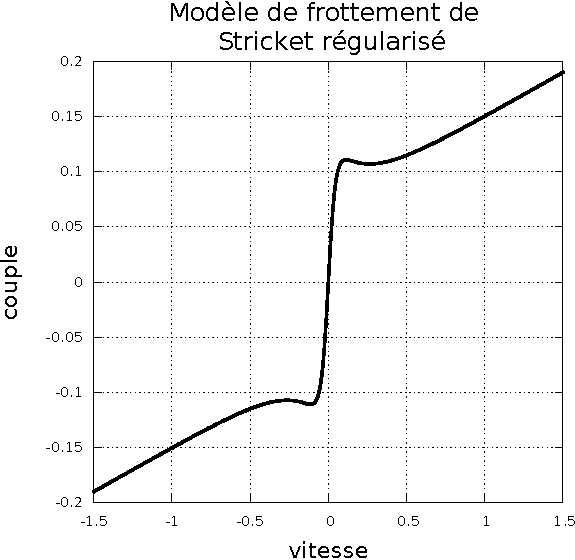
\includegraphics[type=pdf,ext=.pdf,read=.pdf,width=0.5\linewidth]{../plot/friction_model}
        \caption{\label{fig:friction_model}
            Modèle de frottement de Stribeck régularisé à vitesse nulle.
            Les valeurs des différents paramètres du modèle sont ici 
            choisies à titre illustratif.}
    \end{center}
\end{figure}

\subsection{Implémentation}

L'implémentation des calculs dynamiques 
présentés ici repose en grande partie sur la bibliothèque 
logicielle \textit{RBDL} (voir section \ref{sec:model_geometric_rbdl}).
Néanmoins les points suivants en dehors du champ de RBDL
ont été implémentés :
\begin{itemize}
    \item Modèle dynamique inverse en double support.
    \item Gestion des états (actifs ou pas) des points de contact
        et des définitions des contraintes cinématiques.
    \item Construction du problème LCP.
    \item Algorithme général du simulateur. 
        Intégration des équations différentielles de
        la dynamique directe.
    \item Expérimentation de la dynamique impulsive.
    \item Calcul du ZMP.
    \item Réimplémentation partielle de certaines fonctions de
        la bibliothèque RBDL afin prendre en compte l'inertie interne des servomoteurs.
    \item Modélisation des servomoteurs.
        Notons que l'implémentation d'un modèle du jeu mécanique,
        non détaillé ici a été commencé.
\end{itemize}
Le code source écrit en C++ peut être consulté à l'adresse :\\
\url{https://github.com/RhobanProject/Model}\\

